\documentclass[tikz,border=4pt]{standalone}
\usepackage{tikz}\usetikzlibrary{arrows.meta}
\definecolor{nebula}{HTML}{6366F1}\definecolor{spark}{HTML}{14B8A6}
\begin{document}
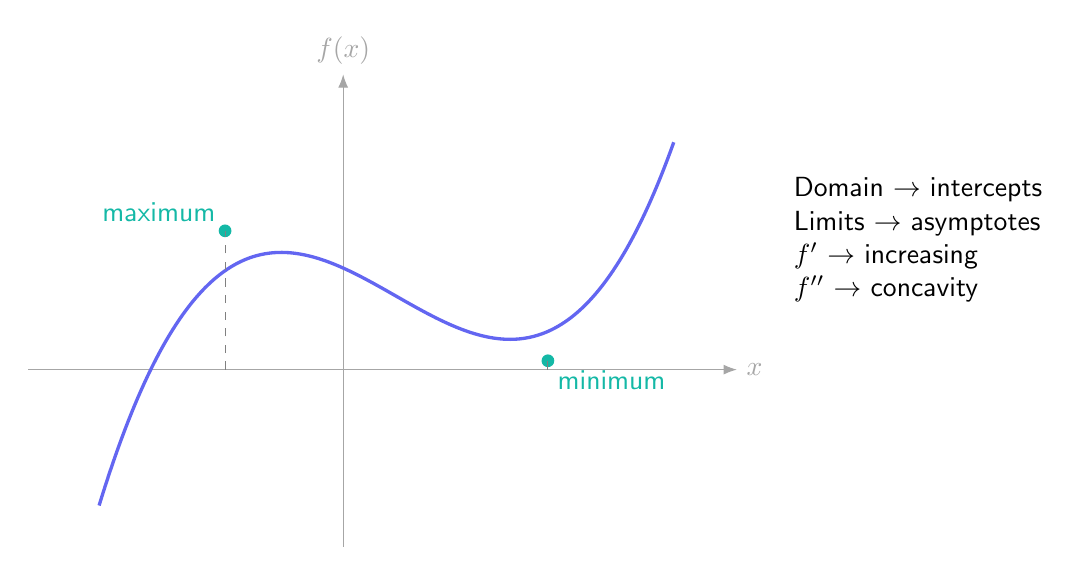
\begin{tikzpicture}[x=1cm,y=.75cm,font=\sffamily,>=Latex]
  \draw[->,gray!70] (-4,0)--(5,0) node[right] {$x$}; \draw[->,gray!70] (0,-3)--(0,5) node[above] {$f(x)$};
  \draw[domain=-3.1:4.2,samples=180,very thick,nebula] plot (\x,{0.12*(\x+2)*(\x-1)*(\x-3)+1});
  \fill[spark] (-1.5,2.35) circle(2.3pt) node[above left] {maximum}; \fill[spark] (2.6,.15) circle(2.3pt) node[below right] {minimum};
  \draw[dashed,gray] (-1.5,0)--(-1.5,2.35) (2.6,0)--(2.6,.15);
  \node[align=left] at (7.3,2.2) {Domain $\rightarrow$ intercepts\\Limits $\rightarrow$ asymptotes\\$f'$ $\rightarrow$ increasing\\$f''$ $\rightarrow$ concavity};
\end{tikzpicture}
\end{document}
